% -- content from the PSfragPrologue option --
%auto-ignore (makes arXiv.org ignore this file)
% This file replaces labels in an EPS graphic by LaTeX macros,
% i.e. it should be accompanied by an EPS file (Shadow_9-psfrag.eps). 
\def\PFGstripminus-#1{#1}%
\def\PFGshift(#1,#2)#3{\raisebox{#2}[\height][\depth]{\hbox{%
  \ifdim#1<0pt\kern#1 #3\kern\PFGstripminus#1\else\kern#1 #3\kern-#1\fi}}}%
\providecommand{\PFGstyle}{}%
% -- end of PSfragPrologue option --
\begin{psfrags}%
\psfragscanon%
%
% psfrag replacement commands
\psfrag{alpha}[cl][cl]{\PFGstyle $\alpha/M_\bullet$}%
\psfrag{beta}[bc][bc]{\PFGstyle $\beta/M_\bullet$}%
\psfrag{x0}[tc][tc]{\PFGstyle $0$}%
\psfrag{x21}[tc][tc]{\PFGstyle $2$}%
\psfrag{x41}[tc][tc]{\PFGstyle $4$}%
\psfrag{x61}[tc][tc]{\PFGstyle $6$}%
\psfrag{x81}[tc][tc]{\PFGstyle $8$}%
\psfrag{xm21}[tc][tc]{\PFGstyle $-2$}%
\psfrag{xm41}[tc][tc]{\PFGstyle $-4$}%
\psfrag{xm61}[tc][tc]{\PFGstyle $-6$}%
\psfrag{xm81}[tc][tc]{\PFGstyle $-8$}%
\psfrag{y0}[cr][cr]{\PFGstyle $0$}%
\psfrag{y21}[cr][cr]{\PFGstyle $2$}%
\psfrag{y41}[cr][cr]{\PFGstyle $4$}%
\psfrag{y61}[cr][cr]{\PFGstyle $6$}%
\psfrag{y81}[cr][cr]{\PFGstyle $8$}%
\psfrag{ym21}[cr][cr]{\PFGstyle $-2$}%
\psfrag{ym41}[cr][cr]{\PFGstyle $-4$}%
\psfrag{ym61}[cr][cr]{\PFGstyle $-6$}%
\psfrag{ym81}[cr][cr]{\PFGstyle $-8$}%
%
% Figure:
\resizebox{12cm}{!}{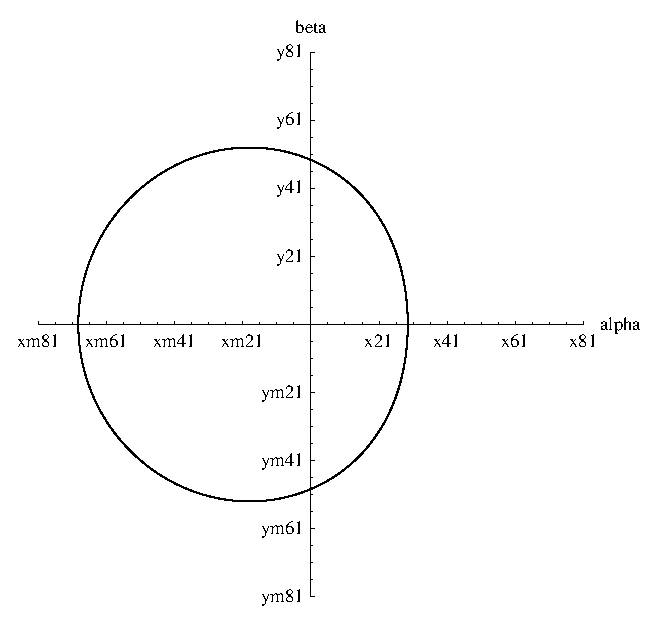
\includegraphics{Shadow_9-psfrag.eps}}%
\end{psfrags}%